\documentclass[journal,12pt,twocolumn]{IEEEtran}

\usepackage{setspace}
\usepackage{gensymb}
\singlespacing
\usepackage[cmex10]{amsmath}

\usepackage{amsthm}
\usepackage{commath}
\usepackage{mathrsfs}
\usepackage{txfonts}
\usepackage{stfloats}
\usepackage{bm}
\usepackage{cite}
\usepackage{cases}
\usepackage{subfig}

\usepackage{longtable}
\usepackage{multirow}

\usepackage{enumitem}
\usepackage{mathtools}
\usepackage{steinmetz}
\usepackage{tikz}
\usepackage{circuitikz}
\usepackage{verbatim}
\usepackage{tfrupee}
\usepackage[breaklinks=true]{hyperref}
\usepackage{graphicx}
\usepackage{tkz-euclide}

\usetikzlibrary{calc,math}
\usepackage{listings}
    \usepackage{color}                                            %%
    \usepackage{array}                                            %%
    \usepackage{longtable}                                        %%
    \usepackage{calc}                                             %%
    \usepackage{multirow}                                         %%
    \usepackage{hhline}                                           %%
    \usepackage{ifthen}                                           %%
    \usepackage{lscape}     
\usepackage{multicol}
\usepackage{chngcntr}

\DeclareMathOperator*{\Res}{Res}

\renewcommand\thesection{\arabic{section}}
\renewcommand\thesubsection{\thesection.\arabic{subsection}}
\renewcommand\thesubsubsection{\thesubsection.\arabic{subsubsection}}

\renewcommand\thesectiondis{\arabic{section}}
\renewcommand\thesubsectiondis{\thesectiondis.\arabic{subsection}}
\renewcommand\thesubsubsectiondis{\thesubsectiondis.\arabic{subsubsection}}


\hyphenation{op-tical net-works semi-conduc-tor}
\def\inputGnumericTable{}                                 %%

\lstset{
%language=C,
frame=single, 
breaklines=true,
columns=fullflexible
}
\begin{document}

\newcommand{\BEQA}{\begin{eqnarray}}
\newcommand{\EEQA}{\end{eqnarray}}
\newcommand{\define}{\stackrel{\triangle}{=}}
\bibliographystyle{IEEEtran}
\raggedbottom
\setlength{\parindent}{0pt}
\providecommand{\mbf}{\mathbf}
\providecommand{\pr}[1]{\ensuremath{\Pr\left(#1\right)}}
\providecommand{\qfunc}[1]{\ensuremath{Q\left(#1\right)}}
\providecommand{\sbrak}[1]{\ensuremath{{}\left[#1\right]}}
\providecommand{\lsbrak}[1]{\ensuremath{{}\left[#1\right.}}
\providecommand{\rsbrak}[1]{\ensuremath{{}\left.#1\right]}}
\providecommand{\brak}[1]{\ensuremath{\left(#1\right)}}
\providecommand{\lbrak}[1]{\ensuremath{\left(#1\right.}}
\providecommand{\rbrak}[1]{\ensuremath{\left.#1\right)}}
\providecommand{\cbrak}[1]{\ensuremath{\left\{#1\right\}}}
\providecommand{\lcbrak}[1]{\ensuremath{\left\{#1\right.}}
\providecommand{\rcbrak}[1]{\ensuremath{\left.#1\right\}}}
\theoremstyle{remark}
\newtheorem{rem}{Remark}
\newcommand{\sgn}{\mathop{\mathrm{sgn}}}
\providecommand{\abs}[1]{\vert#1\vert}
\providecommand{\res}[1]{\Res\displaylimits_{#1}} 
\providecommand{\norm}[1]{\lVert#1\rVert}
%\providecommand{\norm}[1]{\lVert#1\rVert}
\providecommand{\mtx}[1]{\mathbf{#1}}
\providecommand{\mean}[1]{E[ #1 ]}
\providecommand{\fourier}{\overset{\mathcal{F}}{ \rightleftharpoons}}
%\providecommand{\hilbert}{\overset{\mathcal{H}}{ \rightleftharpoons}}
\providecommand{\system}{\overset{\mathcal{H}}{ \longleftrightarrow}}
	%\newcommand{\solution}[2]{\textbf{Solution:}{#1}}
\newcommand{\solution}{\noindent \textbf{Solution: }}
\newcommand{\cosec}{\,\text{cosec}\,}
\providecommand{\dec}[2]{\ensuremath{\overset{#1}{\underset{#2}{\gtrless}}}}
\newcommand{\myvec}[1]{\ensuremath{\begin{pmatrix}#1\end{pmatrix}}}
\newcommand{\mydet}[1]{\ensuremath{\begin{vmatrix}#1\end{vmatrix}}}
\numberwithin{equation}{subsection}
\makeatletter
\@addtoreset{figure}{problem}
\makeatother
\let\StandardTheFigure\thefigure
\let\vec\mathbf
\renewcommand{\thefigure}{\theproblem}
\def\putbox#1#2#3{\makebox[0in][l]{\makebox[#1][l]{}\raisebox{\baselineskip}[0in][0in]{\raisebox{#2}[0in][0in]{#3}}}}
     \def\rightbox#1{\makebox[0in][r]{#1}}
     \def\centbox#1{\makebox[0in]{#1}}
     \def\topbox#1{\raisebox{-\baselineskip}[0in][0in]{#1}}
     \def\midbox#1{\raisebox{-0.5\baselineskip}[0in][0in]{#1}}
\vspace{3cm}
\title{Assignment 5}
\author{Savarana Datta - AI20BTECH11008}
\maketitle
\newpage
\bigskip
\renewcommand{\thefigure}{\theenumi}
\renewcommand{\thetable}{\theenumi}
Download all python codes from 
\begin{lstlisting}
https://github.com/SavaranaDatta/EE3900/blob/main/EE3900_As5/codes/EE3900_As5.py
\end{lstlisting}
%
Download latex-tikz codes from 
%
\begin{lstlisting}
https://github.com/SavaranaDatta/EE3900/blob/main/EE3900_As5/EE3900_As5.tex
\end{lstlisting}
\section{Problem(Quadratic Forms Q.2.5)}
Find the area of the region in the first quadrant enclosed by x-axis, line $\myvec{1 & -\sqrt{3}}\vec{x}=0$ and the circle $\vec{x}^\top\vec{x}=4$.
\section{Solution}
Let $\vec{A}$ be the point of intersection of the line $\myvec{1 & -\sqrt{3}}\vec{x}=0$ and the circle $\vec{x}^\top\vec{x}=4$.
\begin{align}
    \vec{A}=\lambda\myvec{1\\ \frac{1}{\sqrt{3}}}
\end{align}
As $\vec{A}$ lie in the $1^{st}$ quadrant
\begin{align}
\label{eq}
    \lambda > 0
\end{align}
As $\vec{A}$ lie on the circle, we have
\begin{align}
    \vec{A}^\top\vec{A}&=4\\
    \lambda^2+\frac{\lambda^2}{3}&=4\\
    \implies \lambda&=\pm \sqrt{3} 
\end{align}
From \ref{eq},
\begin{align}
    \lambda = \sqrt{3}
\end{align}
Therefore 
\begin{align}
    \vec{A}=\myvec{\sqrt{3}\\1}
\end{align}
Let $\vec{B}$ be the point of intersection of x-axis and the circle.
\begin{align}
    \vec{B}=\lambda_1\myvec{1\\0}
\end{align}
As $\vec{B}$ lie on the positive side of the x-axis 
\begin{align}
    \label{eq1}
    \lambda_1>0
\end{align}
As $\vec{B}$ lie on the circle, we have
\begin{align}
    \vec{B}^\top \vec{B}&=4\\
    \lambda_1^2&=4\\
    \implies \lambda_1 &=\pm 2 
\end{align}
From \ref{eq1}
\begin{align}
    \lambda_1&=2\\
    \implies \vec{B}&=\myvec{2\\0}
\end{align}
The angle($\theta$) of the sector AOB is 
\begin{align}
    \cos{\theta}&=\frac{\vec{A}^{\top}\vec{B}}{\norm{\vec{A}}\norm{\vec{B}}}\\
    &=\frac{2\sqrt{3}}{2\times 2}\\
    &=\frac{\sqrt{3}}{2}\\
    \implies \theta &= 30^{\degree}
\end{align}
\begin{align}
    \text{Area of the sector}&=\brak{\frac{\theta}{360^{\degree}}}\pi r^2\\
    &= \frac{\pi}{3}
\end{align}
\begin{figure}[!h]
 \centering
 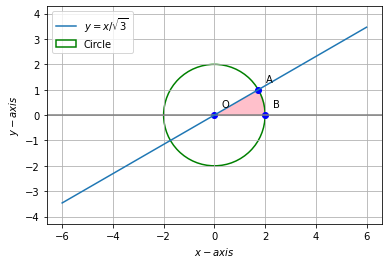
\includegraphics[width=\columnwidth]{fig.png}
 \caption{Reference plot}
 \label{plot}
\end{figure}
\end{document}
